\section{The NSI Hypothesis}\label{sec:constraining}
In this section, we will constrain the four NSI parameters $\ett$, $\emt$, $\eem$, and $\eet$. As we shall see, the impacts of NSI mainly manifest
themselves at \si{\GeV} energies, causing us to bring back DeepCore and PINGU. We will consider the results obtained from these three detectors separately as well as jointly.

\subsection{\texorpdfstring{$\chi^2$}{Chi-squared} Minimization}
\label{sec:nsi_chi2}
For our analyses, we define our $\chi^2$ as
\begin{align}\label{eq:chisq_NSI}
    \chi^{2}(\hat{\theta},\alpha,\beta, \kappa)=\sum_{ijk} \frac{\left(N^\text{th}-N^\text{data}\right)_{ijk}^{2}}
    {\left(\sigma^\text{data}_{ijk}\right)^{2} + \left(\sigma^\text{syst}_{ijk}\right)^{2}}+ 
    \frac{(1-\alpha)^2}{\sigma_\alpha^2} + \frac{\beta^2}{\sigma_\beta^2}\,
\end{align}
where we minimize over the model parameters $\hat{\theta} \in \{\dm, \theta_{23}, \epsilon\}$, the penalty terms $\alpha$ and $\beta$, and the free parameter $\kappa$.
$N_{ijk}^\text{th}$ is the expected number of events from theory in bin $\{i,j,k\}$, where $i$ denotes the $\Ereco$ bin, $j$ denotes the $\zreco$ bin,
and $k$ denotes the event-type bin, i.e. track or cascade. 
$N_{ijk}^\text{data}$ is the observed number of events in that bin. $\sigma^\text{data}_{ijk}$ is the experimental uncertainty, and $\sigma^\text{syst}_{ijk}$ the uncorrelated systematic
uncertainty.

In our simulations of $N_{ijk}^\text{th}$, we set all standard oscillation parameters to their current best-fit values of Eq.~\ref{eq:PINGUparams}, 
except for $\dm[31]$ and $\theta_{23}$
which we vary over their $3\sigma$ limits \SIrange{2.435e-3}{2.598e-3}{\eV\squared} and \SIrange{40.1}{51.7}{\degree}, respectively~\cite{nufit}.

We set $\sigma_\alpha = 0.25$ as the atmospheric flux normalization error, and $\sigma_\beta = 0.05$ as the zenith angle slope error~\cite{hondapaper}. 
The observed event number has an associated Poissonian uncertainty $\sigma_{ijk}^\text{data} = \sqrt{N_{ijk}^\text{data}}$.
For IceCube, the event count takes the form
\begin{align}
    N^\text{th}_{ij} = \alpha\left[1+\beta (0.5 + \zreco_i )\right] N_{ij}(\hat{\theta})\,,
\end{align}
with $N_{ij}(\hat{\theta})$ from Eq.~\ref{eq:ICevents}. Here, we allow the event distribution to rotate around the median cosine-zenith of $\zreco = -0.5$. 
The event index $k$ is omitted since we only have track events for IceCube.

For DeepCore and PINGU, and the event count takes the form
\begin{align}
    N^\text{th}_{ijk} = \alpha\left[1+\beta \zreco_i \right] N_{ijk}(\hat{\theta}) + \kappa N_{ijk}^{\mu_{atm}}\,,
\end{align}
with $N_{ijk}(\hat{\theta})$ from Eq.~\ref{eq:MCevents}. $N_{ijk}^{\mu_{atm}}$ is the muon background, which is left to float freely in the DeepCore analysis.
The detectors experience an uncorrelated systematic error, which comes from the muon background, 
i.e. events misclassified as muons from 
$\nm$ interactions rather than from pion decay. For the DeepCore analysis, we will have to consider this background when calculating the events.
For IceCube events, we scan a higher energy range where the muon background can be neglected. For the PINGU events, the IceCube detector is 
expected to be able to act as a veto for this background. Thus, the error introduced from the muon background is expected by the collaboration 
to be negligible~\cite{PINGUletter}.
The background at PINGU can be considered negligible to first order~\cite{PINGUdata}, and we thus put $\kappa=0$ when calculating the PINGU $\chi^2$.
For DeepCore and PINGU, the median cosine-zenith is $\zreco = 0$, and we allow the event count to rotate around this point.

We treat the uncorrelated systematic uncertainties differently for each detector. For IceCube, we set $\sigma_{ij}^\text{syst} = f\sqrt{N_{ij}^\text{data}}$.
We consider best, normal, and worst-case scenarios in IceCube using
$f=5\%$, $10\%$, and $15\%$ respectively. For PINGU, we use the same form but instead use $f=0\%$, $3\%$, and $5\%$.
For DeepCore, we use the provided systematic error distribution which accounts for uncertainties in the finite MC statistics and the data-driven 
muon background estimate~\cite{DC2019data}. This is summarized in Table~\ref{table:syst_errors}.
{\renewcommand{\arraystretch}{1.2}
\begin{table}
   \centering
   \begin{tabular}{lccc}
      \hline \hline
      Experiment & Best case & Baseline & Worst case \\
      \hline
      IceCube & $5\%$ & $10\%$ & $15\%$ \\
      PINGU & $0\%$ & $3\%$ & $5\%$ \\
      \hline \hline
   \end{tabular}
   \caption{Our definition of the best, baseline, and worst case scenarios considered in each experiment, modelled by $\sigma_{ijk}^\text{syst} = f\sqrt{N_{ijk}^\text{data}}$ with $f$ from the table.
   We do not consider different DeepCore scenarios because her systematic error distribution is already provided in the data release~\cite{DC2019data}.}\label{table:syst_errors}
\end{table}

For the joint analysis, we follow the parameter goodness-of-fit prescription~\cite{maltoni2003} and construct the joint $\chi^2$ as 
\begin{align}\label{eq:joint_chisq}
    \chi^2_\text{joint} = \sum_\text{exp}\chi^2_\text{exp} - \chi^2_\text{exp,min}\,
\end{align}
with test statistic $\chi^2_\text{joint,min}$. The $\Delta \chi^2_\text{joint}$ is then $\Delta \chi^2_\text{joint} = \chi^2_\text{joint} - \chi^2_\text{joint,min}$.

\subsection{Constraining the NSI parameters}\label{sec:constraining_NSI}
We let each of the four NSI parameters considered assume a value, while keeping the other three fixed at zero. We consider the following ranges of values for each parameter:
\begin{align}
   -0.07 \le &\, \ett \le 0.07 \nonumber \\
   -0.03 \le &\, \emt \le 0.03 \nonumber \\
   -0.3 \le &\, \eem \le 0.3 \nonumber \\
   -0.3 \le &\, \eet \le 0.3 \nonumber \\
\end{align}
After the oscillation parameters $\dm[31]$ and $\theta_{23}$ have been marginalized out, we plot $\Delta \chi^2$ for each of the four NSI parameters in Fig.~\ref{fig:3D_NO}. 
The results are shown in Fig.~\ref{fig:IC_3D} and summarized in Tables~\ref{table:IC_DC_results} and~\ref{table:PINGU_joint_results}. Each region is bounded
by the best and worst-case scenario, as defined in Table~\ref{table:syst_errors}, while the middle line is the baseline scenario. We again emphasize that 
no uncertainty scenarios are considered for DeepCore, since they already provided in the data release~\cite{DC2019data}.

Comparing the PINGU and the DeepCore results in Fig.~\ref{fig:3D_NO}, we note that the best-fit for each NSI parameter for the PINGU experiment is expected to be zero. This is because the `data' we generated during 
the PINGU simulations assume no NSI since they have yet to be observed in nature. This introduces a non-NSI bias in all joint analyses, which include PINGU
since PINGU has stronger statistics than DeepCore and will thus pull the joint $\chi^2$ towards $\epsilon =0$.
Moreover, we see that we can expect PINGU to be sensitive to systematic uncertainty, especially when constraining $\eem$ and $\eet$ from the negative side.

\begin{figure}
   \begin{center}
      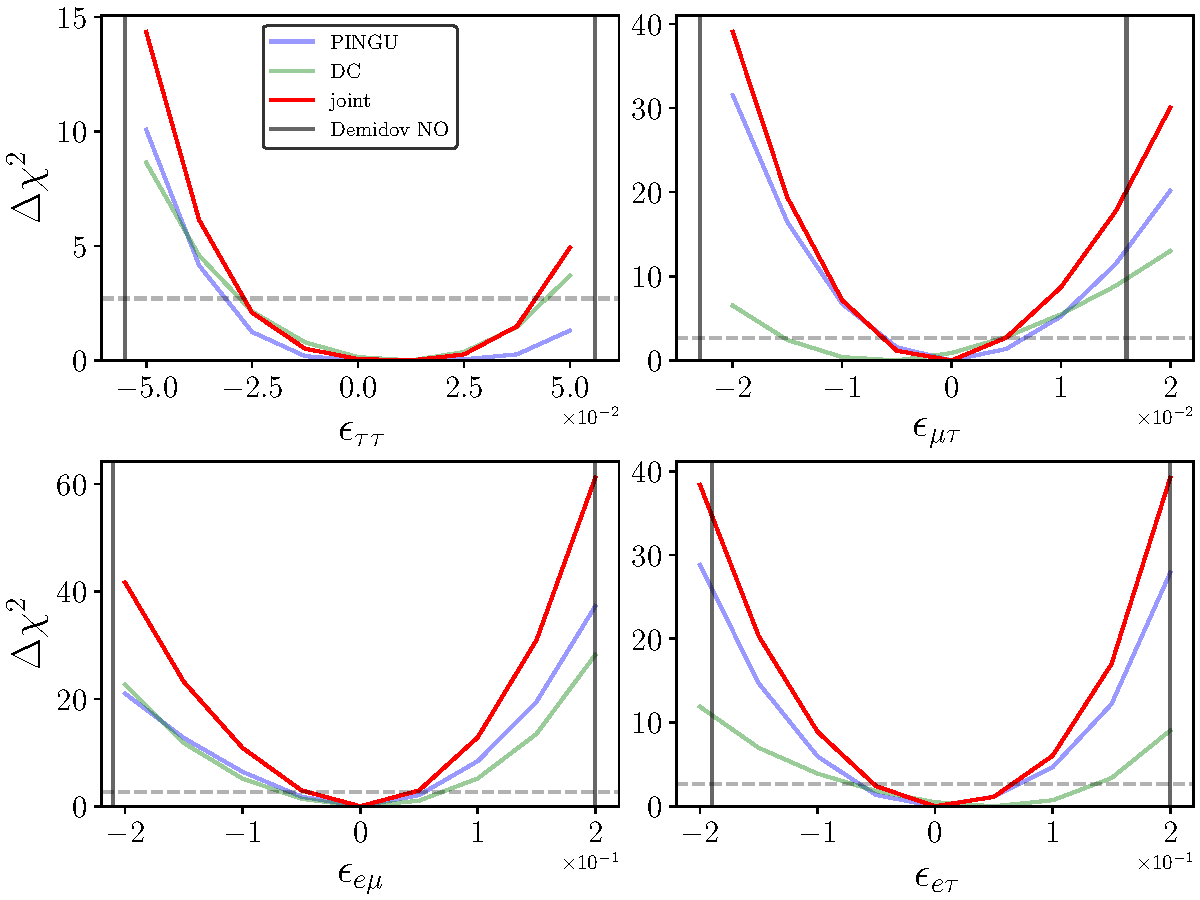
\includegraphics[scale = 0.7]{figures/joint_3D_NO.pdf}
      \caption{Confidence regions for PINGU and DeepCore scenarios listed in Table~\ref{table:syst_errors}, with their joint $\Delta \chi^2$ in maroon. $\dm[31]$ and $\theta_{23}$ and have been marginalized out, and all other NSI 
      parameters not shown in each panel are fixed to zero. 
      IceCube tracks only reveal $\emt$, and are displayed separately in Fig.~\ref{fig:IC_3D}. Dotted lines are the 90\% and $3\sigma$ CL levels.}\label{fig:3D_NO}
   \end{center}
\end{figure} 
\begin{figure}
   \begin{center} 
      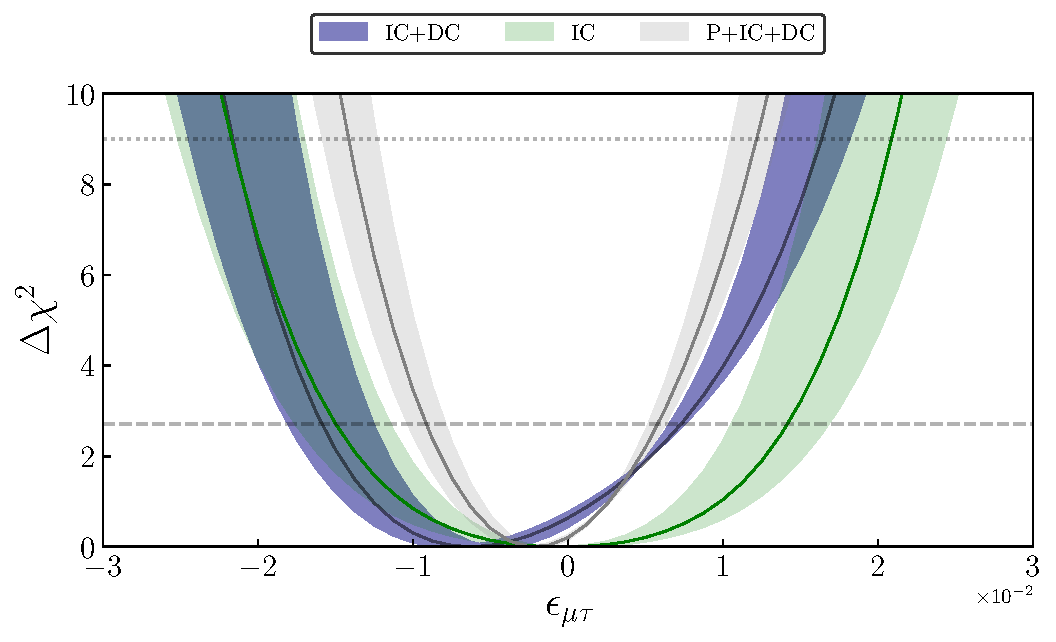
\includegraphics[width=0.8\textwidth]{figures/PID_3D_emt.pdf}
      \caption{$\emt$ $\Delta \chi^2$ regions for scenarios as defined in Table~\ref{table:syst_errors}.
    $\dm[31]$ and $\theta_{23}$ and have been marginalized out, and all other NSI 
    parameters other than $\emt$ are fixed to zero. Dotted lines are the 90\% and $3\sigma$ CL levels.
    The zones contain the three uncertainty scenarios considered, and we see that the inclusion of PINGU is expected 
    to drastically make the bound on $\emt$ more stringent.
    }\label{fig:IC_3D}
   \end{center}
\end{figure}

{\renewcommand{\arraystretch}{1.0}
 \begin{table}
   \begin{center}
      \begin{tabular}{lcc}
         \hline
         Parameter & Best 90\% CL & Best $3\sigma$\\
         \hline & \multicolumn{2}{c}{IceCube}  \\
         $\emt$ &  [-0.012, 0.011] &  [-0.017, 0.016] \\\\
         & \multicolumn{2}{c}{DeepCore}\\ [0.3em]
         $\ett$ &  [-0.054, 0.067] &  [-0.089, 0.10] \\
         $\emt$ &  [-0.029, 0.0070] &  [-0.041, 0.026] \\
         $\eem$ &  [-0.12, 0.15] &  [-0.23, 0.24] \\
         $\eet$ &   [-0.084, 0.15] &  [-0.19, 0.21] \\\\
         &\multicolumn{2}{c}{IceCube + DeepCore} \\
         $\emt$ &  [-0.013, 0.0070] &  [-0.017, 0.013] \\
         \hline
         \vspace{2em}
      \end{tabular}
      \begin{tabular}{lcc}
         \hline
         Parameter & Baseline 90\% CL & Baseline $3\sigma$ \\
         \hline & \multicolumn{2}{c}{IceCube}  \\
         $\emt$ &  [-0.015, 0.014] &  [-0.022, 0.021] \\\\
         & \multicolumn{2}{c}{DeepCore}\\ [0.3em]
         $\ett$ &  [-0.054, 0.067] &  [-0.089, 0.10] \\
         $\emt$ &  [-0.029, 0.0070] &  [-0.041, 0.026] \\
         $\eem$ &  [-0.12, 0.15] &  [-0.23, 0.24] \\
         $\eet$ &   [-0.084, 0.15] &  [-0.19, 0.21] \\\\
         &\multicolumn{2}{c}{IceCube + DeepCore}\\
         $\emt$ &  [-0.016, 0.0070] &  [-0.022, 0.016] \\
         \hline
         \vspace{2em}
      \end{tabular}
      \begin{tabular}{lcc}
         \hline
         Parameter & Worst 90\% CL & Worst $3\sigma$\\
         \hline & \multicolumn{2}{c}{IceCube}  \\
         $\emt$ &  [-0.018, 0.017] &  [-0.025, 0.024] \\\\
         & \multicolumn{2}{c}{DeepCore}\\ [0.3em]
         $\ett$ &  [-0.054, 0.067] &  [-0.089, 0.10] \\
         $\emt$ &  [-0.029, 0.0070] &  [-0.041, 0.026] \\
         $\eem$ &  [-0.11, 0.15] &  [-0.23, 0.24] \\
         $\eet$ &   [-0.084, 0.15] &  [-0.188, 0.212] \\\\
         &\multicolumn{2}{c}{IceCube + DeepCore}\\
         $\emt$ &  [-0.018, 0.0070] &  [-0.024, 0.018] \\
         \hline
      \end{tabular}
      \caption{IceCube and DeepCore results from the $\Delta \chi^2$ in Fig.~\ref{fig:IC_3D}. $\dm[31]$ and $\theta_{23}$ have been marginalized out, and all other NSI parameters other than the one shown for each row are set to zero. Best, baseline, and worst refer to 
      the systematic uncertainty scenarios considered as in Table~\ref{table:syst_errors}.}\label{table:IC_DC_results}
   \end{center}
\end{table}

\begin{table}
   \centering
   \begin{tabular}{lcc}
      \hline
      Parameter & Best 90\% CL & Best $3\sigma$\\
      \hline & \multicolumn{2}{c}{PINGU} \\
      $\ett$ &  [-0.044, 0.051] &  [-0.062, 0.069] \\
      $\emt$ &  [-0.008, 0.009] &  [-0.014, 0.017] \\
      $\eem$ &  [-0.079, 0.081] &   [-0.16, 0.138] \\
      $\eet$ &  [-0.079, 0.098] &  [-0.148, 0.161] \\\\
      & \multicolumn{2}{c}{DeepCore + PINGU} \\
      $\ett$ &  [-0.036, 0.046] &  [-0.056, 0.064] \\
      $\emt$ &  [-0.0090, 0.0060] &  [-0.015, 0.013] \\
      $\eem$ &   [-0.060, 0.077] &  [-0.13, 0.13] \\
      $\eet$ &  [-0.052, 0.095] &  [-0.11, 0.14] \\\\
      & \multicolumn{2}{c}{IceCube + DeepCore + PINGU}  \\
      $\emt$ &  [-0.0080, 0.0050] &  [-0.012, 0.011] \\
      \hline
      %\vspace{0.5em}
   \end{tabular}
   \begin{tabular}{lcc}
      \hline 
      Parameter & Baseline 90\% CL & Baseline $3\sigma$\\
      \hline & \multicolumn{2}{c}{PINGU} \\
      $\ett$ &  [-0.046, 0.054] &  [-0.065, 0.073] \\
      $\emt$ &   [-0.0090, 0.010] &  [-0.015, 0.018] \\
      $\eem$ &  [-0.11, 0.094] &  [-0.20, 0.16] \\
      $\eet$ &   [-0.10, 0.11] &  [-0.19, 0.18] \\\\
      & \multicolumn{2}{c}{DeepCore + PINGU} \\
      $\ett$ &    [-0.038, 0.048] &  [-0.058, 0.067] \\
      $\emt$ &    [-0.010, 0.0060] &  [-0.016, 0.014] \\
      $\eem$ &    [-0.071, 0.086] &  [-0.15, 0.14]  \\
      $\eet$ &   [-0.061, 0.10] &  [-0.13, 0.16] \\\\
      & \multicolumn{2}{c}{IceCube + DeepCore + PINGU}  \\
      $\emt$ &  [-0.009, 0.0060] &  [-0.014, 0.012] \\
      \hline
      %\vspace{0.5em}
   \end{tabular}
   \begin{tabular}{lcc}
      \hline 
      Parameter & Worst 90\% CL & Worst $3\sigma$\\
      \hline & \multicolumn{2}{c}{PINGU} \\
      $\ett$ &  [-0.049, 0.057] &   [-0.07, 0.078] \\
      $\emt$ &   [-0.01, 0.011] &   [-0.017, 0.02] \\
      $\eem$ &   [-0.137, 0.11] &   [-0.228, 0.18] \\
      $\eet$ &  [-0.132, 0.125] &  [-0.226, 0.196] \\\\
      & \multicolumn{2}{c}{DeepCore + PINGU} \\
      $\ett$ &   [-0.039, 0.050] &    [-0.060, 0.070] \\
      $\emt$ &  [-0.011, 0.0070] &  [-0.017, 0.015] \\
      $\eem$ &  [-0.082, 0.097] &  [-0.168, 0.16] \\
      $\eet$ &  [-0.067, 0.11] &  [-0.15, 0.17] \\\\
      & \multicolumn{2}{c}{IceCube + DeepCore + PINGU}  \\
      $\emt$ &   [-0.010, 0.0060] &  [-0.016, 0.013] \\
      \hline
   \end{tabular}
   \caption{PINGU and joint results from the $\Delta \chi^2$ in Fig.~\ref{fig:3D_NO}. $\dm[31]$ and $\theta[23]$ have been marginalized out, and all other NSI parameters other than the one shown for each row are set to zero.
   Best, baseline, and worst refer to 
   the systematic uncertainty scenarios considered as in Table~\ref{table:syst_errors}.}\label{table:PINGU_joint_results}
\end{table}


\begin{table}
   \begin{center}
   \begin{tabular}{lccc}
           \hline \hline & \multicolumn{3}{c} {\text {Best fit}} \\
           \cline { 2 - 4 } Parameter & $\dm[31]$ & $\theta_{23}$  & $\epsilon$  \\
           \hline \multicolumn{3}{c} {\hspace{2.5cm} DeepCore }  \\[0.1em]
           $\ett$ &  2.435 & 47.84 & 0.0125 \\
           $\emt$ &  2.435 & 43.97 & -0.005 \\
           $\eem$ &  2.435 & 43.97 & 0 \\
           $\eet$ &  2.435 & 43.97  & 0.05 \\\\
           \multicolumn{3}{c} {\hspace{2.5cm} IceCube } \\
           $\emt$ &  2.435 & 51.70 & 0 \\
           \multicolumn{3}{c} {\hspace{2.5cm} IceCube + DeepCore } \\
           $\emt$ &  2.517 & 43.97 & -0.01 \\
           \hline
           \hline
   \end{tabular}
   \end{center}
   \caption{Best fit points for $\dm[31]$ and $\theta_{23}$ are given in units of $\si{10^{-3}\eV\squared}$ and
   degrees, respectively.}\label{table:bestfit}
\end{table}

We compare our results to a similar analysis performed on the same DeepCore dataset in~\cite{demidov}. In that publication, 
the constraints found at 90\% CL were 
\begin{align}\label{eq:demidov}
   -0.055 <&\, \ett < 0.056 \nonumber \\
   -0.023 <&\, \emt < 0.016 \nonumber \\
   -0.21 <&\, \eem < 0.20 \nonumber \\
   -0.19 <&\, \eet < 0.20\,.
\end{align}
Comparing~\ref{eq:demidov} to our results from Table~\ref{table:IC_DC_results} at 90\% CL, namely
\begin{align}\label{eq:DC_results}
   -0.054 <&\, \ett < 0.067 \nonumber \\
   -0.029 <&\, \emt < 0.0070 \nonumber \\
   -0.12 <&\, \eem < 0.15 \nonumber \\
   -0.084 <&\, \eet < 0.15\,,
\end{align}
we see that our results for $\eem$, $\eet$ are more stringent, while the results for $\emt$ and $\ett$ are similar but more lenient. It is worth noting that the 
results from~\cite{demidov} are have been obtained by including more systematic uncertainties, such as the spectral index, hadron production, and baryon resonance. 
However, the overall flux normalization in~\cite{demidov} is 20\%, while we opted for a slightly higher figure of 25\%, which could compensate for the exclusion of the 
statistical uncertainties mentioned.

Using the baseline case of 3\% systematic uncertainty at 90\% CL, we find from Table~\ref{table:PINGU_joint_results}, that our predictions for the proposed PINGU detector are
\begin{align}\label{eq:P_results}
   -0.049 <&\, \ett < 0.057 \nonumber \\
   -0.010 <&\, \emt < 0.011 \nonumber \\
   -0.137 <&\, \eem < 0.11 \nonumber \\
   -0.132 <&\, \eet < 0.125\,,
\end{align}
which displays an improvement over the DeepCore results in Eq.~\ref{eq:DC_results}, except for $\eet$ which is worse.

Finally, the joint results for $\emt$ using IceCube and DeepCore from~\ref{table:PINGU_joint_results} at 90\% CL are
\begin{align}\label{eq:ID_result}
   -0.016 <&\, \emt < 0.0070\,,
\end{align}
and when combining IceCube, DeepCore, and PINGU, the 90\% CL constraint on $\emt$ in our baseline scenario is predicted to be
\begin{align}\label{eq:PID_result}
   -0.010 <&\, \emt < 0.0060\,,
\end{align}
which is more stringent for $\emt>0$ than the result in~\cite{deepcoreNSI}.

 \begin{figure}[t]
   \begin{center}
      \begin{subfigure}{0.44\textwidth}
         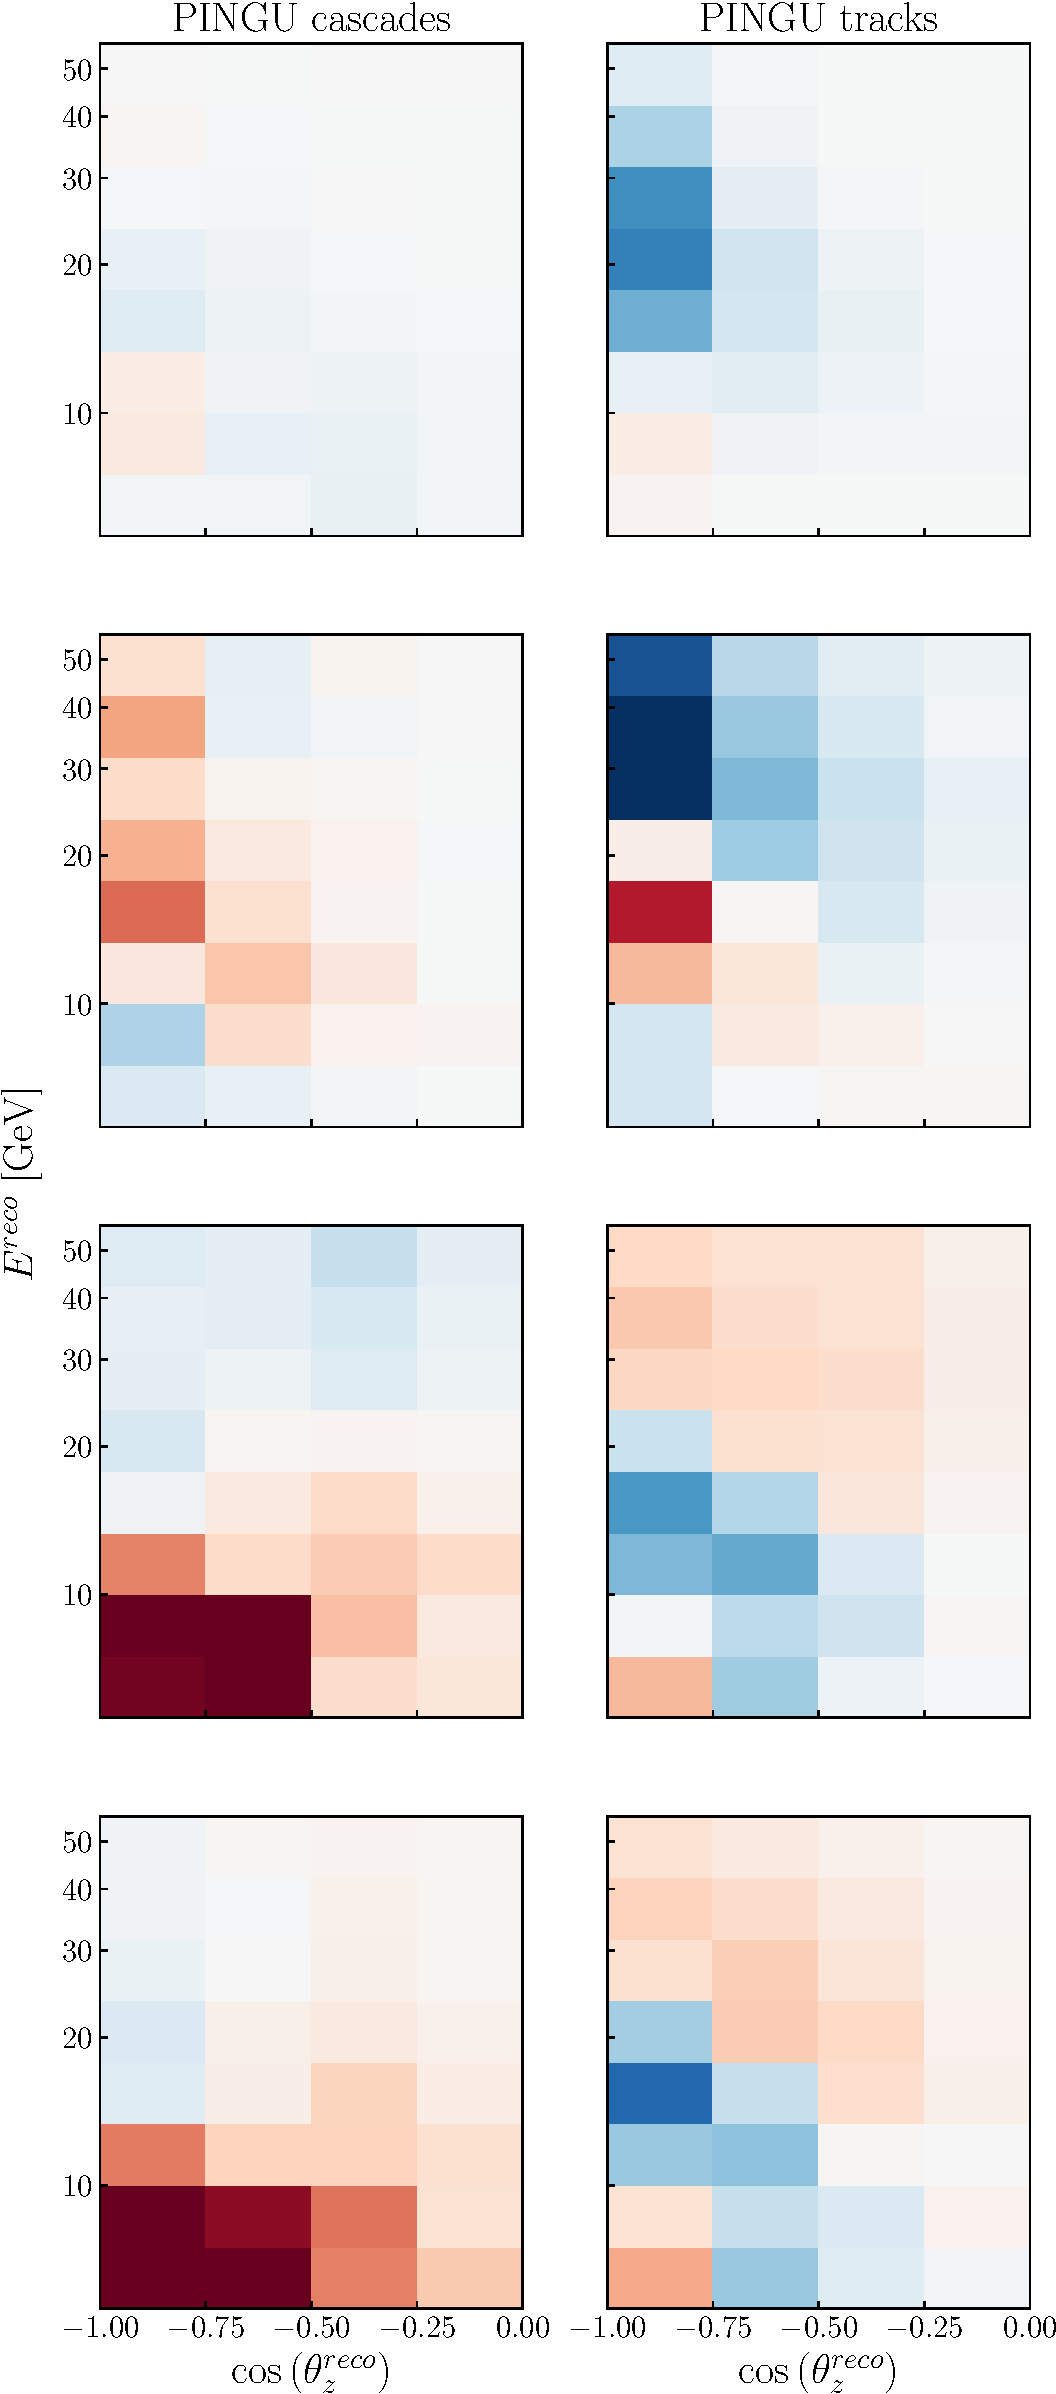
\includegraphics[width=1\linewidth]{figures/PINGU_event_pulls.pdf}
         \caption{PINGU}\label{fig:PINGU_event_pulls}
      \end{subfigure}
      \begin{subfigure}{0.54\textwidth}
         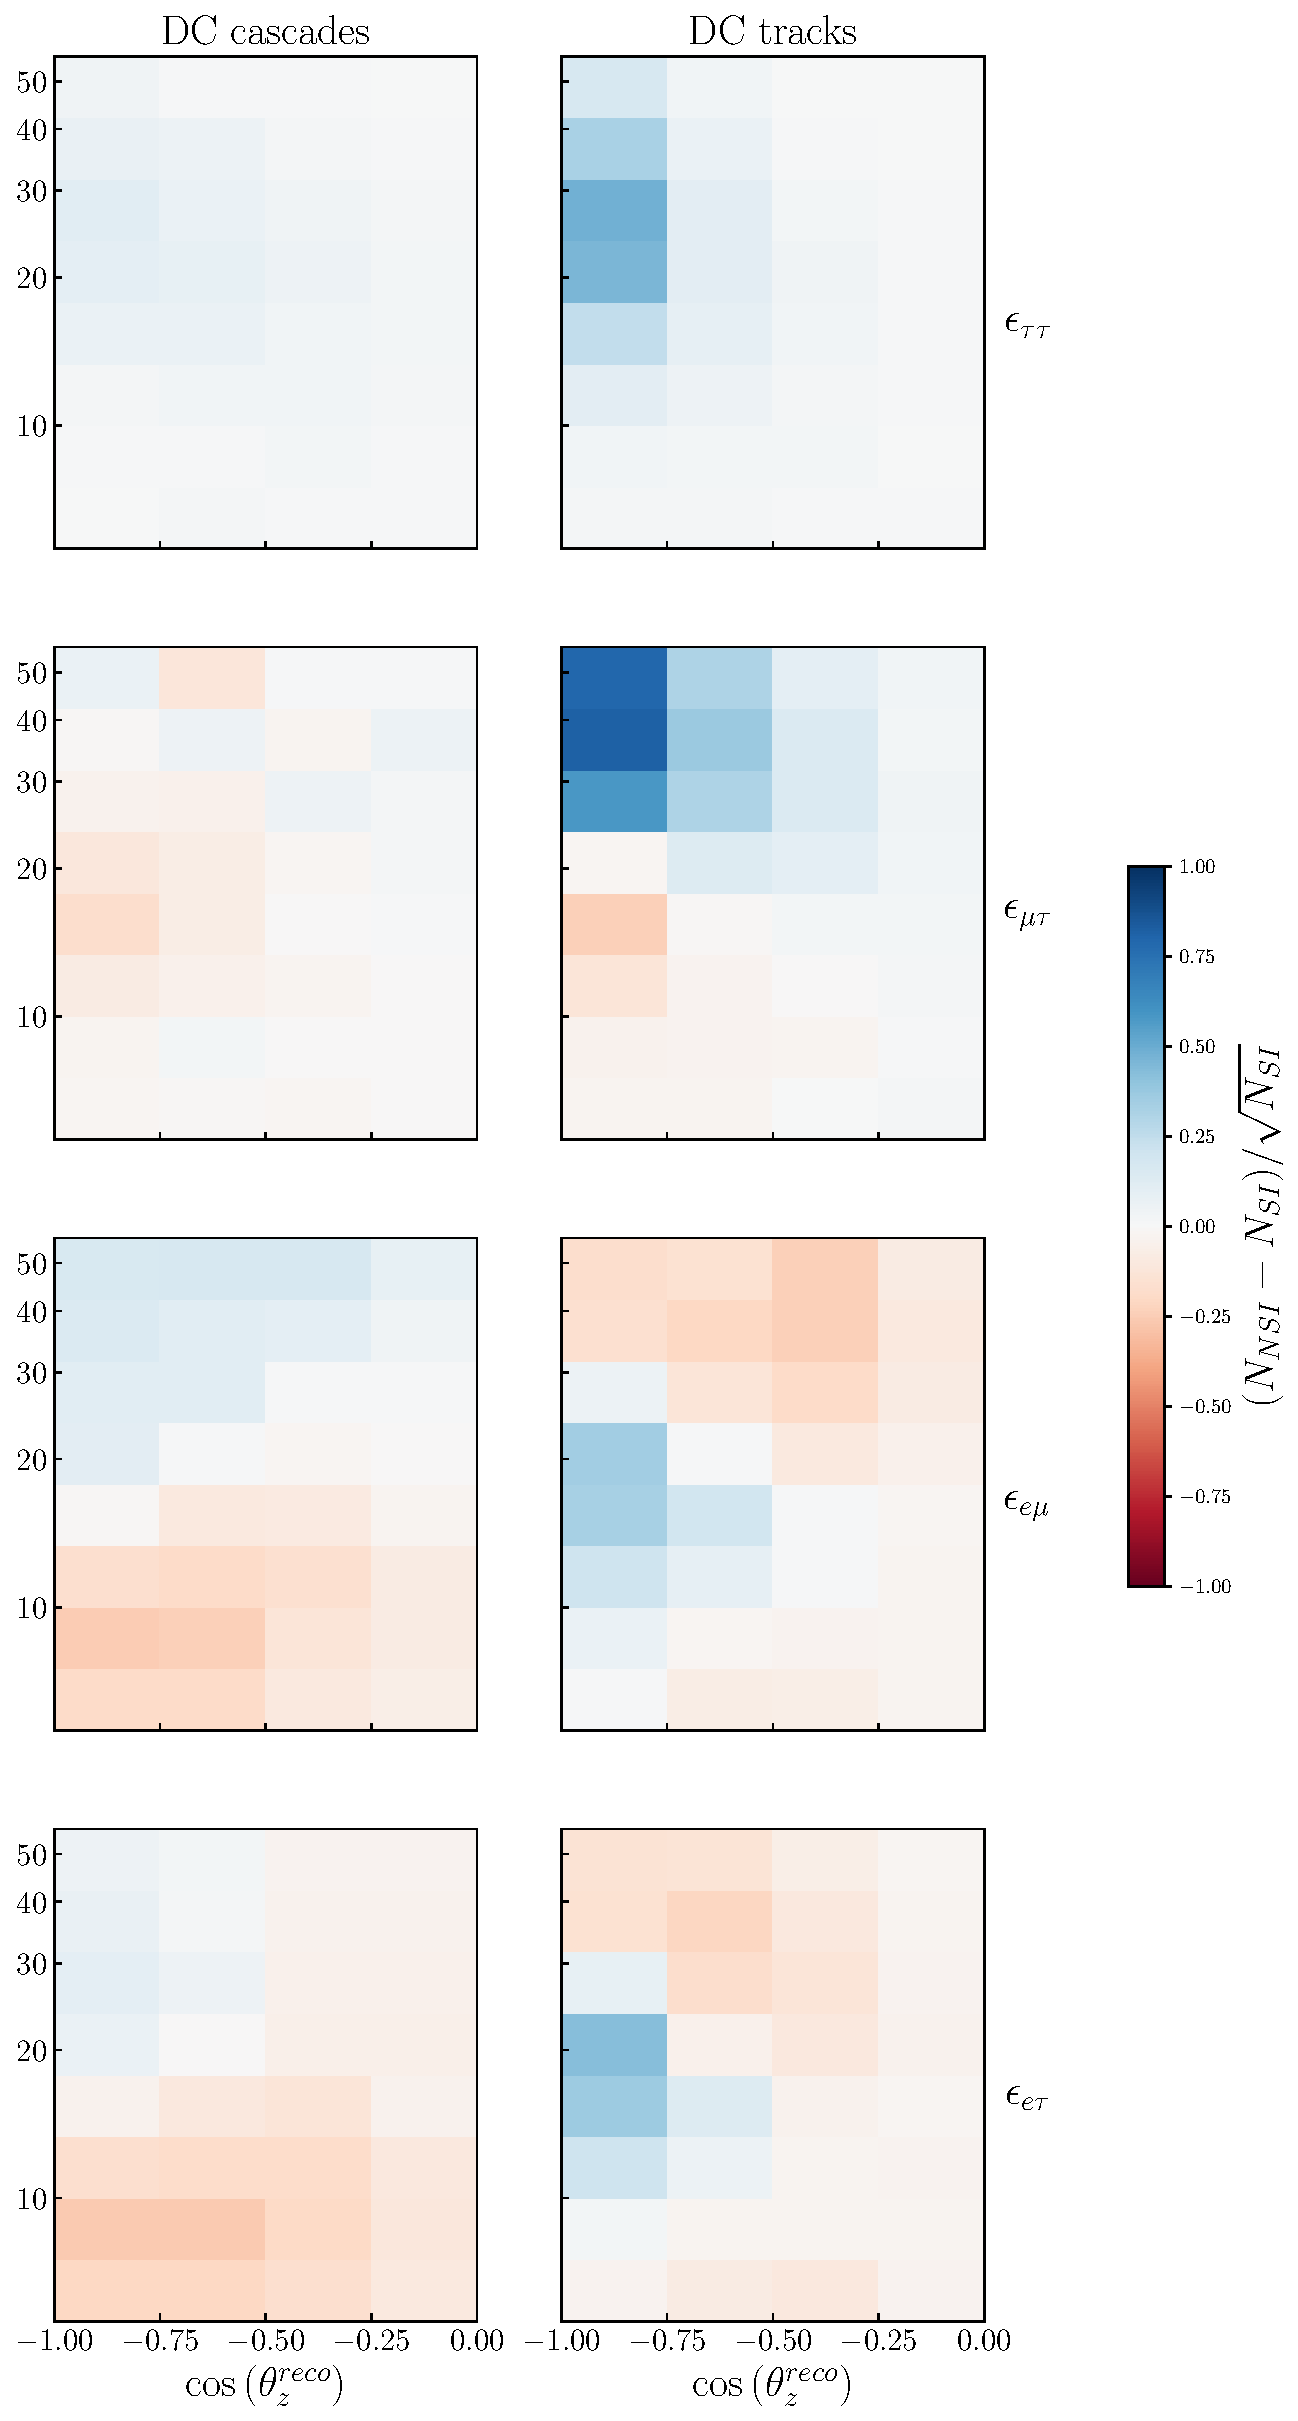
\includegraphics[width=1\linewidth]{figures/DC_event_pulls.pdf}
         \caption{DeepCore}\label{fig:DC_event_pulls}
      \end{subfigure}
    \end{center}
   \caption{Expected pulls of the form $(N_{NSI} - N_{SI})/\sqrt{N_{SI}}$ for PINGU and DeepCore after 3 years of data. 
   Each row has only one NSI non-zero parameter, with the first row having $\ett= -0.07$, second $\emt = -0.03$, third $\eem = -0.3$, and fourth $\eet = -0.3$.
   We clearly see the increased statistics of the PINGU detector, especially in cascade events. The low values of $\ett$ and $\emt$ produce a weak pull in DeepCore,
   while PINGU can be expected to observe multiple regions of strong pulls for $\emt$, $\eem$, and $\eet$.}\label{fig:event_pulls}
\end{figure}

We plot the event pull $(N_{NSI} - N_{SI})/\sqrt{N_{SI}}$ where $N_{(N)SI}$ are the numbers of expected events
assuming (non-)standard interactions in Fig.~\ref{fig:event_pulls}. This gives the normalized difference in the
number of expected events at the detector and illustrates the expected sensitivity of DeepCore for the NSI parameters.

Now we will compare the probability plots with the final event counts in DeepCore. It is not enough to only study the effect at probability level, since that is in true quantities. 
Since the detector data comes in reconstructed quantities, it might be the case that a feature at probability level gets averaged out in the reconstruction, and not showing up at all in the data. 
In general, features showing at probability level are can be 
averaged out at reconstruction if they occur in the rapidly oscillating part of single-digit \si{\GeV} energies. 

The top right panel shows a surplus of DeepCore track events at \SIrange{20}{30}{\GeV} for through-going neutrinos when we turn on $\ett$. This is what we expected from the bottom right panel in Fig.~\ref{fig:emt_ett_probs}, where we saw that we had an increase in $\anm$ survival probability at \SIrange{20}{40}{\GeV}. 

The third right panel shows the expected event pull for $\eem$. Comparing with the probabilities in Fig.~\ref{fig:eem_eet_probs}, we see that the surplus of the $\anm$ survival in the \SIrange{20}{30}{\GeV} and the deficit above \SI{40}{\GeV} is intact, while the \SI{10}{\GeV} $\nm$ deficit is completely averaged out.

There is no reason for us to assume that only one NSI parameter exists in Nature, unless we impose a symmetry on the gauge group which generates NSI. For example, the matter potential matrix in our Hamiltonian from Eq.~\eqref{eq:V_matrix} is diagonal since the 
interaction Lagrangian respects lepton flavor conservation. So ideally, we would simulate a grid where all NSI parameters are allowed to vary, 
but this is not feasible. Thus, we take we set $\ett = 0$ and let $\emt,\eem,\eet$ vary, along with $\dm[31]$ and $\theta_{23}$. We let $\ett=0$ because we saw that it did not influence the other parameters. 
We then marginalize out the standard oscillation parameters and one of the NSI parameters and plot the remaining two in Fig.~\ref{fig:PINGU_2D}. We see that the pairs $\eem - \emt$ and $\eet - \emt$ are symmetrical. 
Hence, we can see that no relationship exists between them. With $\eet - \eem$, however, the contours are assuming a different shape. The contour allows positive values of $\eet$ and $\eem$ to a greater degree than mixed or negative values.
Thus, we can draw the conclusion that, given $\ett = 0$, PINGU might expect to observe that $\eem$ and $\emt$ are anti-correlated while we expect no significant correlation
to be be seen between the pairs $\emt - \eem$, and $\emt - \eet$. This is consistent with our observation of the effect of these parameters on $\Pme$ in  Fig.~\ref{fig:eem_eet_prob}, from which we 
saw that $\eem$ and $\eet$ strongly affect $\Pme$ for single-digit \si{\GeV} energies.

\begin{figure}
   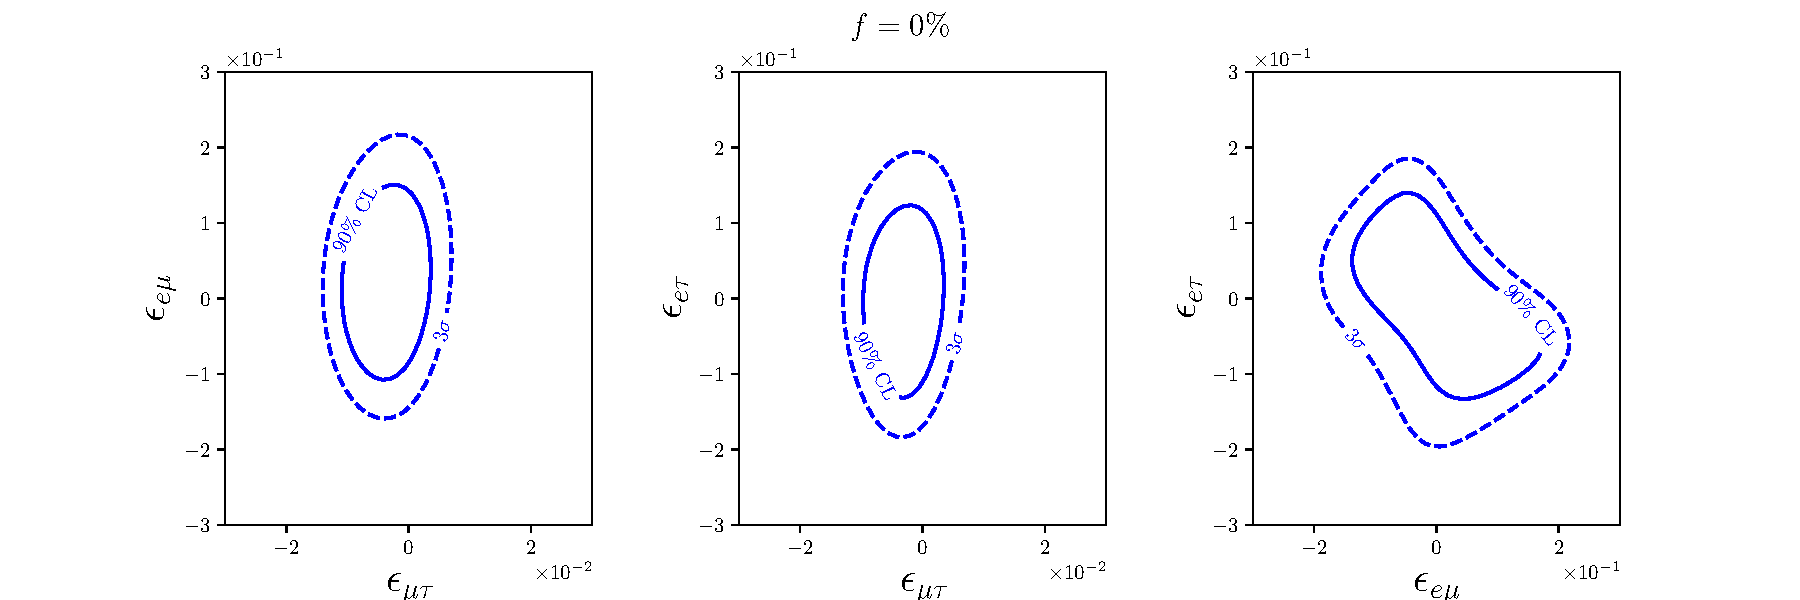
\includegraphics[scale=0.5]{figures/PINGU_2D_all_f0.pdf}
   \caption{Allowed regions for some of the NSI parameters after three years of PINGU data, assuming no uncorrelated systematic error. All plots are made with $\ett = 0$. The two
   standard oscillation parameters $\dm[31]$ and $\theta_{23}$ along with the one NSI parameter not shown have been marginalized out. We observe an anti-correlation between $\eem$ and $\eet$,
   consistent with our observation of the effect of these parameters on $\Pme$ in  Fig.~\ref{fig:eem_eet_prob}.
   The values of the standard oscillation parameters 
   are taken from NuFit~\cite{nufit}.}\label{fig:PINGU_2D}
\end{figure}